\documentclass[border=10pt]{standalone}

\usepackage{tikz}
\usepackage{tikzsymbols}
\usetikzlibrary{calc,patterns,shapes.geometric}

\def\centerarc[#1](#2)(#3:#4:#5){\draw[#1] ($(#2)+({#5*cos(#3)},{#5*sin(#3)})$) arc (#3:#4:#5);}

\begin{document}
	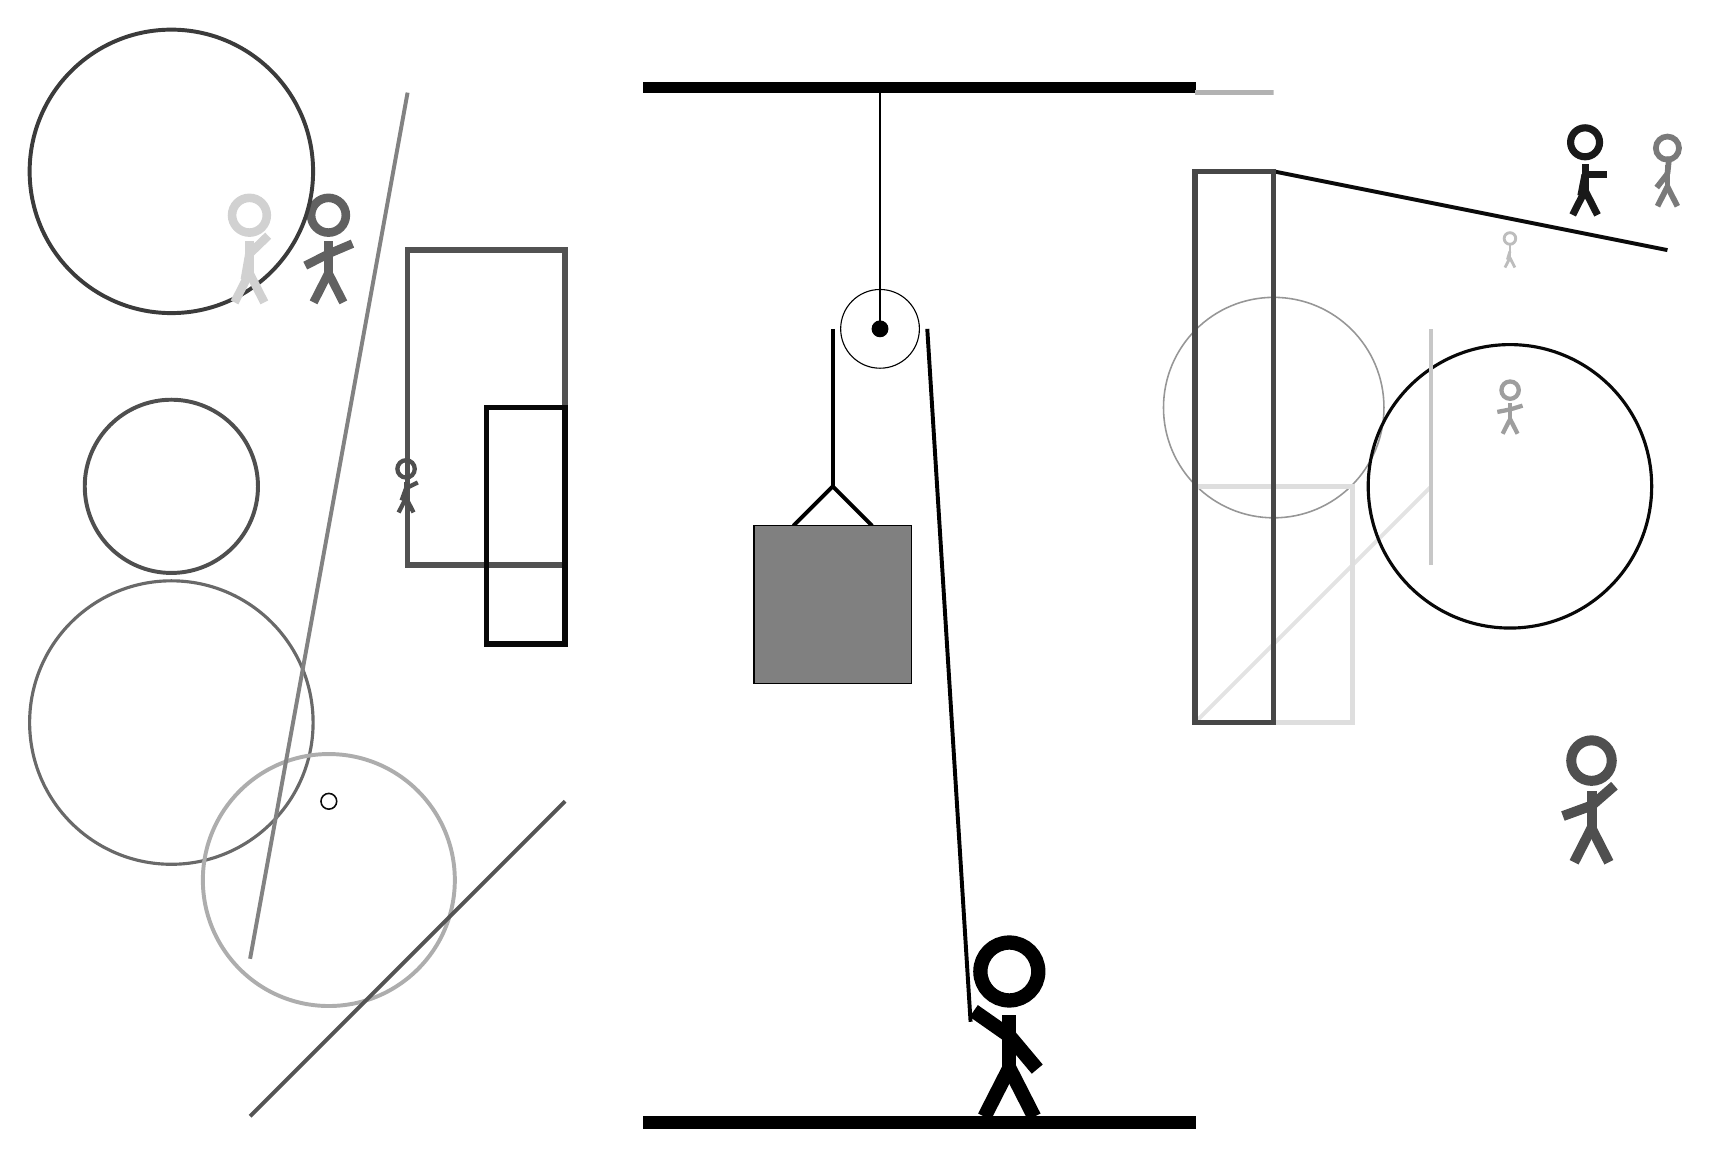
\begin{tikzpicture}
		%%%%% START %%%%%
		
		\draw[fill=black] (-2, 10) rectangle (5, 10.125);
		
		\draw (1, 7) circle (0.5);
		\draw[fill=black] (1, 7) circle (0.1);
		\draw (1, 10) -- (1, 7);
		
		\draw [line width=0.2mm, color=black!96](-6, 1) circle (0.1);
		
		\node[line width=0.4mm, color=black!62] at (-6, 8) {\Strichmaxerl[6][27][23]};
		\draw [line width=0.4mm, color=black!59](-8, 2) circle (1.8);
		\draw [line width=0.5mm, color=black!32](-6, 0) circle (1.6);
		
		\draw [line width=0.2mm, color=black!41](6, 6) circle (1.4);
		\draw[line width=0.7mm, color=black!68] (-3, 8) rectangle (-5, 4);
		
		\draw[line width=0.5mm, color=black!11](8, 5) -- (5, 2);
		
		\draw [line width=0.5mm, color=black!77](-8, 9) circle (1.8);
		\node[line width=0.6mm, color=black!69] at (10, 1) {\Strichmaxerl[7][20][41]};
		
		\node[line width=0.2mm, color=black!18] at (-7, 8) {\Strichmaxerl[6][80][44]};
		\draw[line width=0.5mm, color=black!96](6, 9) -- (11, 8);
		\draw[line width=0.7mm, color=black!30] (5, 10) rectangle (6, 10);
		\draw [line width=0.4mm, color=black!97](9, 5) circle (1.8);
		
		\draw[line width=0.5mm, color=black!22](8, 4) -- (8, 7);
		\draw[line width=0.5mm, color=black!67](-3, 1) -- (-7, -3);
		\draw[line width=0.7mm, color=black!13] (5, 5) rectangle (7, 2);
		\node[line width=0.4mm, color=black!26] at (9, 8) {\Strichmaxerl[2][73][90]};
		\draw[line width=0.7mm, color=black!72] (6, 2) rectangle (5, 9);
		\node[line width=0.3mm, color=black!90] at (10, 9) {\Strichmaxerl[5][79][0]};
		\node[line width=0.6mm, color=black!38] at (9, 6) {\Strichmaxerl[3][11][17]};
		\node[line width=0.4mm, color=black!52] at (11, 9) {\Strichmaxerl[4][52][84]};
		
		\draw[line width=0.5mm, color=black!49](-5, 10) -- (-7, -1);
		
		\node[line width=0.5mm, color=black!69] at (-5, 5) {\Strichmaxerl[3][70][26]};
		\draw[line width=0.7mm, color=black!97] (-3, 6) rectangle (-4, 3);
		\draw [line width=0.5mm, color=black!69](-8, 5) circle (1.1);
		
		
		\draw[line width=0.5mm] (-0.1, 4.5) -- (0.4, 5.0) -- (0.9, 4.5);
		\draw[fill=black!50] (-0.6, 4.5) rectangle (1.4, 2.5);
		
		\draw[line width=0.5mm] (0.4, 7) -- (0.4, 5.0);
		\centerarc[line width=0.5mm](1, 7)(0:180:0.6);
		\draw[line width=0.5mm](1.6, 7) -- (2.15, -1.8);
		
		\node at (2.6, -1.9) {\Strichmaxerl[10][-35][-50]};
		
		\draw[fill=black] (-2, -3) rectangle (5, -3.15);
		
		%%%%% END %%%%%
	\end{tikzpicture}
\end{document}